
\begin{lemma}{7.2.304}\label{lem:7-2-304}
存在滤过 $A_{n,K}$ 同态
\[
\begin{gathered}
\mathfrak e_a\colon
C([0,1]_s\times L'_0,(\lambda_0,\lambda'_0))\\
\longrightarrow C([0,1]_s\times L'_0,\lambda'_0),
\end{gathered}
\]
以及滤过 $A_{n',K'}$ 同态
\[
\begin{gathered}
\mathfrak E_a\colon
C_a([0,1]_s\times L'_1,
((\lambda_0,\lambda'_0),\lambda'_1))
\longrightarrow
C_a([0,1]_s\times L'_1,(\lambda'_0,\lambda'_1)),\\
j_{[0,1]_s}\colon
C_a([0,1]_s\times L'_1,(\lambda'_0,\lambda'_1))
\longrightarrow
C([0,1]_s\times L'_1,\lambda'_1),
\end{gathered}
\]
满足下列条件：

\par\noindent\textup{(7.2.305.1)}
$\mathfrak e_a$、$\mathfrak E_a$
和 $j_{[0,1]_s}$
分别在
$C([0,1]_s\times L'_0,\lambda'_0)$、
$C_a([0,1]_s\times L'_1,(\lambda'_0,\lambda'_1))$
及 $C([0,1]\times L'_1,\lambda'_1)$
上为恒等映射。

\begin{equation}
\operatorname{Eval}_{s=s_0}\circ\mathfrak e_a
=j_{s=s_0}\circ\operatorname{Eval}_{s=s_0}.
\tag{7.2.305.2}\label{eq:7-2-305-2}
\end{equation}
\begin{equation}
\operatorname{Eval}_{s=s_0}\circ\mathfrak E_a
=j_{s=s_0}\circ\operatorname{Eval}_{s=s_0}.
\tag{7.2.305.3}\label{eq:7-2-305-3}
\end{equation}
\begin{equation}
\operatorname{Eval}_{s=s_0}\circ j_{[0,1]_s}
=j\circ\operatorname{Eval}_{s=s_0}.
\tag{7.2.305.4}\label{eq:7-2-305-4}
\end{equation}
\end{lemma}

可以仿照命题~\ref{prop:7-2-211}
的证明，用障碍理论构造这样的
$\mathfrak e_a$、$\mathfrak E_a$、
$j_{[0,1]_s}$。
后文在“同伦的同伦”的更困难情形中，
会详细展开类似论证，
故此处略去证明。
见引理 7.2.310 与命题 7.2.312 的证明。

由 (7.2.305) 可知，
图式~\ref{diag:7-2-19} 在同伦意义下交换。

\par\medskip\noindent\begin{minipage}{\textwidth}
\centering
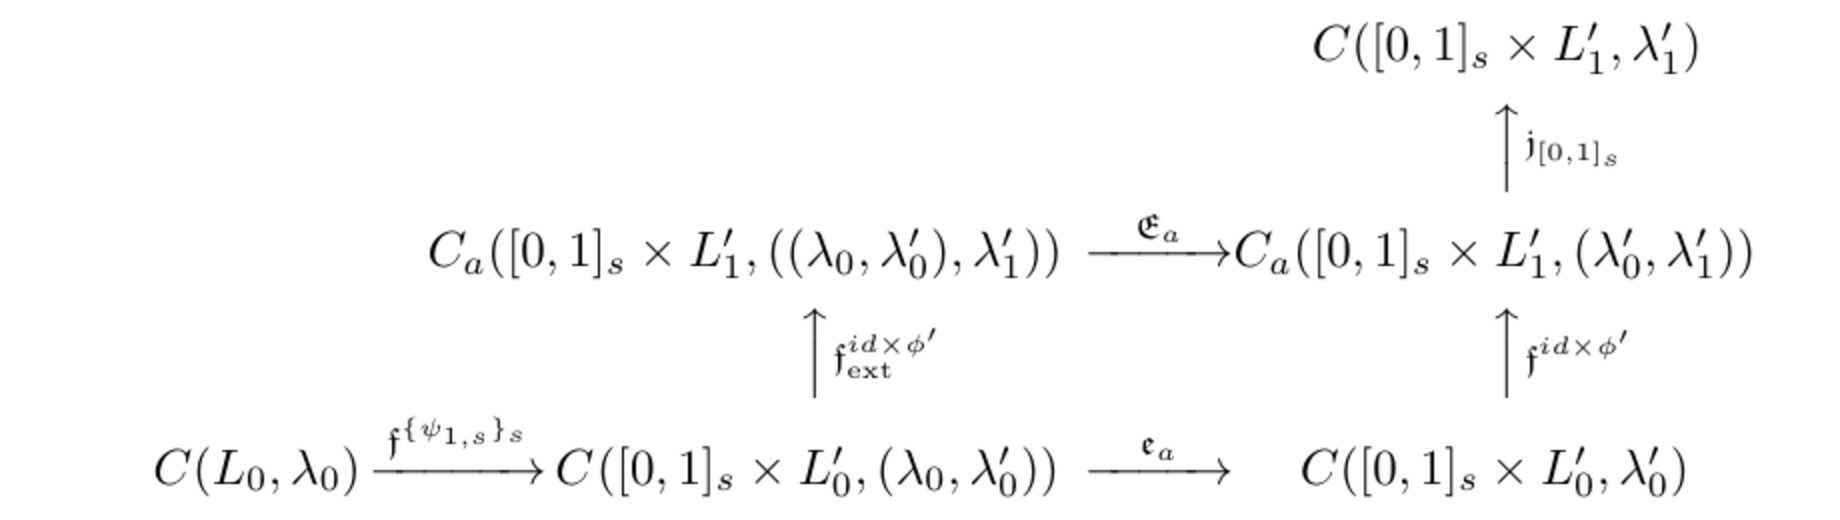
\includegraphics[width=\textwidth]{chapters/ch07-transversality/figures/phys-561-diagram-7-2-19-math-crop.png}
\par{\renewcommand{\thefigure}{7.2.19}\refstepcounter{figure}
\normalfont\bfseries 图式~\thefigure\label{diag:7-2-19}}
\end{minipage}\par\medskip

下面将在引理 7.2.310\translatornote{原书此处写
“引理 7.2.309”；但 7.2.309 是注，
图式~\ref{diag:7-2-19} 两条复合之间的同伦
由引理 7.2.310 给出。}
中具体给出图式~\ref{diag:7-2-19}
的方块中两条复合之间的同伦。
先从不带 $s$ 参数的版本入手。
